\documentclass{report}
\usepackage[utf8]{inputenc}
\usepackage[english]{babel}
\usepackage{multicol}
\usepackage{natbib}
\usepackage{graphicx}
\usepackage{float}
\usepackage{amsfonts}
\usepackage{amssymb}

\author{a.sukachev@lancaster.ac.uk }
\title{GryphonSharp Proposal}
\date{\parbox{\linewidth}{\centering%
    \normalsize \noindent\rule{0.8\textwidth}{0.2pt}
    \vspace*{20pt}\endgraf
    Coordinator: Abe Karnik (a.karnik@lancaster.ac.uk)\endgraf
    Research group: MSc410 (Human Computer Interaction)
}}%hax

\begin{document}

\maketitle

\section{introduction}
Recently, world has been heavily digitized - practically, every aspect of everyday life is in digital form ranging from digital watches to smart houses. With the increasing demand for programming in nearly all science disciplines, need for programming education has risen drastically \citep{MargGoodBern2011wv, jovanovi_digitalization, 7318200}.
Since introduction of Visual Programming environments such as Scratch into education, average performance of students has increased \citep{tsai_2019_improving} while barriers of getting intuition in programming fell down \citep{kelleher_2005_lowering}.
There are a lot of languages out there, which provide constructs and other tools to achieve a given task.



\section{Background}
%Mention little bit more of the research that will be covered. Obviously, the whole purpose of the project is having all this background fused into a working prototype of VPL.

\section{Scope}
Project will cover basic programs without extensive programming features, such as attributes, abstraction or even basic objects. The aim here is to fuse already existing studies of visual programming languages into a working prototype that is capable of producing simple programs, such as guess a number or console calculator.

\section{Application}
Since the invention of C language, computer languages have been tremendous help in many applications. General purpose languages emerged to put extra layer of abstraction on top of "one-at-the-time instruction" assembly language.\citep{10.1145/364063.364092}
As mentioned above by \citep{kelleher_2005_lowering,tsai_2019_improving}, the final prototype of the language can be used in educational purposes

\section{Methodology}
\subsection*{Overview}
Implementing fully functioning programming language that compiles into assembler is a genuinely time-consuming task, which also requires in-depth knowledge of different processor architectures such as ARM, AMD64 and Intel64. For this reason, the project's visual language instead will transpile into C\# Intermediate Language (henceforth IL) using CodeDOM feature of the language.
\subsection*{Visual Editor}
The visual editor, or in this case node editor, will be implemented as a webpage canvas using Konvajs framework.
Konvajs lets you easily serialize and deserialize data and populate the 'code map'. Refer to figure \ref{fig:codemap}.

\begin{figure}[H]
\centering
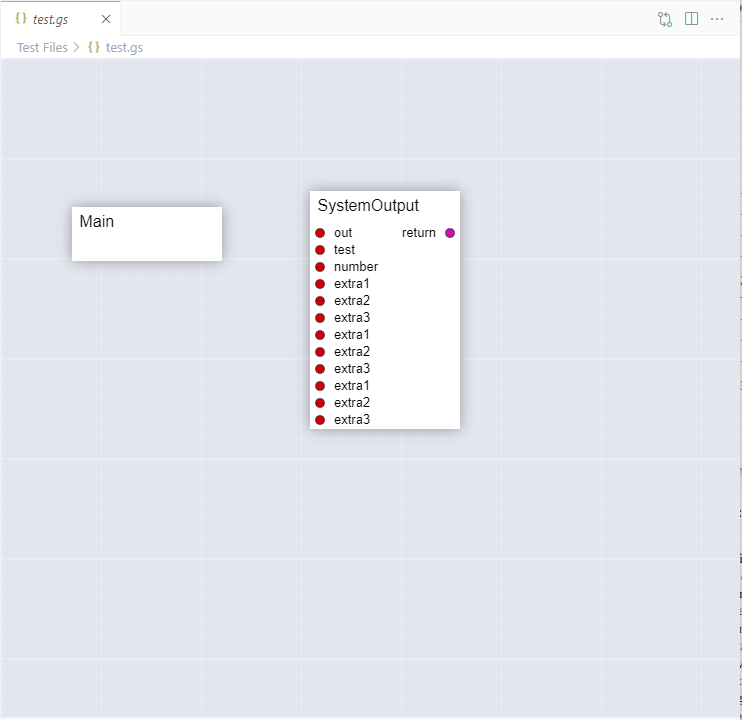
\includegraphics[width=1\textwidth]{codemap.PNG}
\caption{Code Map}
\label{fig:codemap}
\end{figure}

The webpage will be able to serialize all node structure into a JSON file, which will be a source code of a file. This JSON can then be parsed by Transpiler and convert its contents into C\# IL.
The Konvajs framework will be closely tied with Electron app called 'Visual Studio Code' (henceforth VSCode). VSCode 
\subsection*{Transpiler}
As previously stated, the primary purpose of a transpiler is converting source of GryphonSharp-generated JSON files into C\# IL. Transpiler is named 
\subsection*{Language Server}


\section{Time Plan}
Project's time plan will span over 3 months and is represented by Gantt Chart below.

\section{Summary}


\bibliographystyle{plain}
\bibliography{refs}
\end{document}
